\section{Evaluation}
\label{sec:evaluation}

We now evaluate \tritonsort's performance and scalability under
various hardware configurations.

\subsection{Evaluation Environment}

We evaluated \tritonsort on 52 nodes of the cluster described in
Section~\ref{sec:hardware_architecture}.  Each XFS partition is configured with
a single allocation group to prevent file fragmentation across allocation
groups, and is mounted with the \texttt{noatime}, \texttt{attr2},
\texttt{nobarrier}, and \texttt{noquota} flags set.  For this evaluation, the
servers were running Linux 2.6.35.1. Our implementation of \tritonsort is
written in C++.

\subsection{Comparison to Alternatives}

The 100TB Indy GraySort benchmark was introduced in 2009, and hence there are
few systems against which we can compare \tritonsort's performance. The most
recent holder of the Indy GraySort benchmark, DEMSort~\cite{DEMSort}, sorted
slightly over 100TB of data on 195 nodes at a rate of 564 GB per minute.
\tritonsort currently sorts 100TB of data on \tsnodes nodes at a rate of
\tsrate GB per minute, a factor of \tsimprovementfactor improvement in per-node
efficiency.

\subsection{Examining Changes in Balance}

We next examine the effect of changing the cluster's configuration to support
more memory or faster disks. Due to budgetary constraints, we could not
evaluate these hardware configurations at scale. Evaluating
the performance benefits of SSDs is the subject of future work.

In the first experiment, we replaced the 500GB, 7200RPM disks that are used as
the intermediate disks in phase one and the input disks in phase two with
146GB, 15000RPM disks. The reduced capacity of the drives necessitated running
an experiment with a smaller input data set.  To allow space for the logical
disks to be pre-allocated on the intermediate disks without overrunning the
disks' capacity, we decreased the number of logical disks per physical disk by
a factor of two. This doubles the amount of data in each logical disk, but the
experiment's input data set is small enough that the amount of data per logical
disk does not overflow the logical disk's maximum size.

Phase one throughput in these experiments is slightly lower than in subsequent
experiments because the 30-35 seconds it takes to write the last few bytes of
each logical disk at the end of the phase is roughly 10\% of the total runtime
due to the relatively small dataset size.

\begin{table*}
\centering
\caption{\label{table:15k}Effect of increasing speed of intermediate disks
  on a two node, 500GB sort.}
\resizebox{\columnwidth}{!}{%
\begin{tabular}{|c|c|c|c|c|}
\hline
\textbf{Intermediate Disk} & \textbf{Logical Disks}  & \textbf{Phase 1} &
\textbf{Phase 1} & \textbf{Average Write} \\
\textbf{Speed (RPM)} & \textbf{Per Physical Disk} & \textbf{Throughput (MBps)} & \textbf{Bottleneck Stage} & \textbf{Size (MB)}\\
\hline
7200 & 315 & 69.81 &  \writer & 12.6  \\
7200 & 158 & 77.89 &  \writer & 14.0  \\
15000 & 158 & 79.73 &  \ldts  & 5.02 \\
\hline
\end{tabular}%
}
\end{table*}

The results of this experiment are shown in Table~\ref{table:15k}.  We first
examine the effect of decreasing the number of logical disks without increasing
disk speed. Decreasing the number of logical disks increases the average length
of \ldbuffer chains formed by the \ldts; note that most of the time, full
\writerbuffers (14MB) are written to the disks. In addition, halving the number
of logical disks decreases the number of external cylinders that the logical
disks occupy, decreasing maximal seek latency. These two factors combine
together to net a significant (11\%) increase in phase one throughput.

The performance gained by writing to 15000 RPM disks in phase one is much less
pronounced. The main reason for this is that the increase in write speed causes
the \writers to become fast enough that the \ldts exposes itself as the
bottleneck stage. One side-effect of this is that the
\ldts cannot populate \writerbuffers as fast as they become available, so it
reverts to a pathological case in which it always is able to successfully
retrieve a write token and hence continuously writes minimally-filled (5MB)
buffers. Creating a \ldts stage that dynamically adjusts its write size based
on write token retrieval success rate is the subject of future work.


\begin{table}
\centering
\caption{\label{table:bigmem}Effect of increasing the amount of memory per
  node on a two node, 2TB sort.}
\begin{tabular}{|c|c|c|}
\hline
\textbf{RAM Per}  & \textbf{Phase 1}  & \textbf{Average Write} \\
\textbf{Node (GB)} & \textbf{Throughput (MBps)} & \textbf{Size (MB)} \\
\hline
24 & 73.53 & 12.43 \\
48 & 76.45 & 19.21 \\
\hline
\end{tabular}
\end{table}

In the next experiment, we doubled the RAM in two of the machines in our
cluster and adjusted \tritonsort's memory allocation by doubling the size of
each \writerbuffer (from 14MB to 28MB) and using the remaining memory (22GB)
to create additional \ldbuffers. As shown in Table~\ref{table:bigmem},
increasing the amount of memory allows for the creation of longer chains of
\ldbuffers in the \ldts, which in turn causes write sizes to increase. The
increase in write size is not linear in the amount of RAM added; this is likely
because we are approaching the point past which larger writes will not
dramatically improve write throughput.

\subsection{\tritonsort Scalability}

\begin{figure}[T]
    \centering
    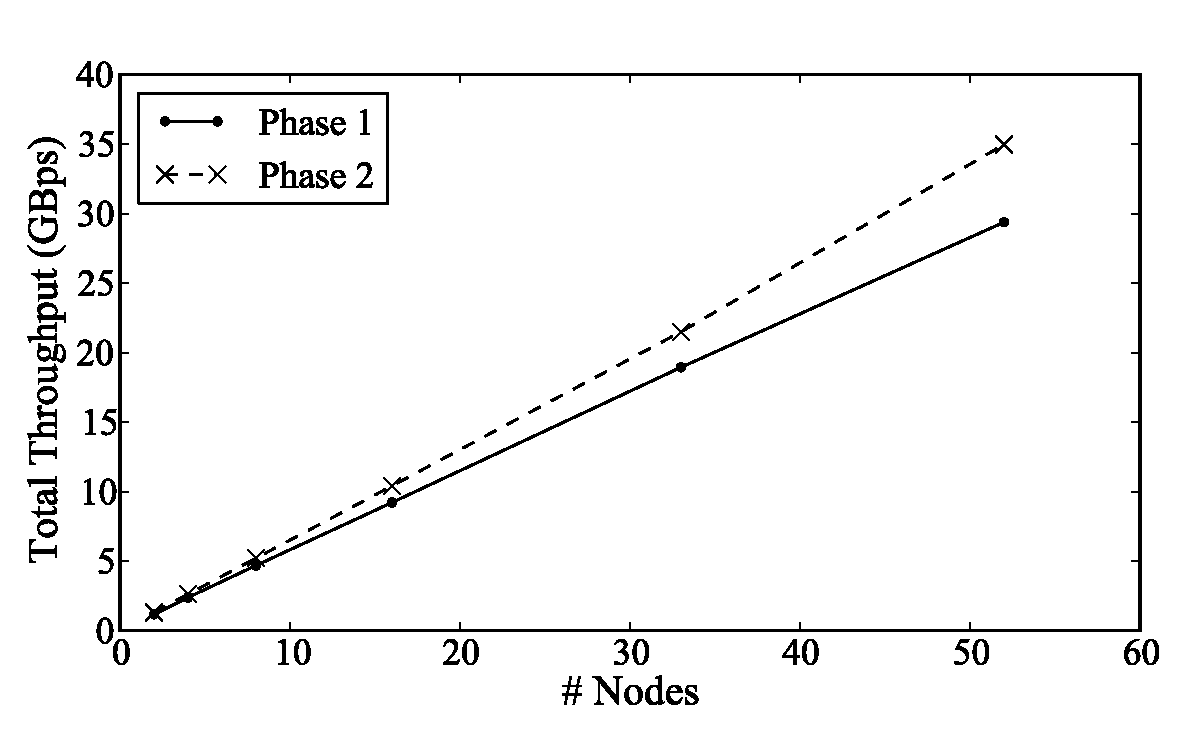
\includegraphics[width=\columnwidth]{tritonsort/graphs/scalability.pdf}

    \caption{\label{fig:scalability}Throughput when sorting 1 TB per node as the number of nodes increases.}
\end{figure}

Figure~\ref{fig:scalability} shows \tritonsort's total throughput when sorting
1 TB per node as the number of nodes increases from 2 to 48. Phase two exhibits
practically linear scaling, which is expected since each node performs phase
two in isolation.  Phase one's scalability is also nearly linear; the slight
degradation in its performance at large scales is likely due to network
variance that becomes more pronounced as the number of nodes increases.

%LocalWords: LocalWords noquota dataset runtime
